\documentclass[10pt,landscape]{article}
\usepackage[margin=0.3in]{geometry}
\usepackage{multicol}
\usepackage{amsmath,amssymb,amsthm}
\usepackage{array}
\usepackage{xcolor}
\usepackage{tikz}
\usetikzlibrary{positioning}
\pagestyle{empty}
\setlength{\parindent}{0pt}
\setlength{\parskip}{2pt}
\setlength{\columnseprule}{0.2pt}

% Define colors
\definecolor{titlecolor}{RGB}{0,51,102}        % Dark blue for main titles
\definecolor{subtitlecolor}{RGB}{153,0,76}     % Dark magenta for subtitles
\definecolor{lemmacolor}{RGB}{0,102,51}        % Dark green for lemma numbers

% Redefine section to use color
\usepackage{titlesec}
\titleformat{\section}
  {\normalfont\Large\bfseries\color{titlecolor}}
  {\thesection}{1em}{}
\titleformat{\subsection}
  {\normalfont\large\bfseries\color{subtitlecolor}}
  {\thesubsection}{1em}{}

% Command for lemma numbers
\newcommand{\lem}[1]{\textbf{\color{lemmacolor}#1}}

\begin{document}
\footnotesize
\begin{multicols}{3}

\section*{Logic}
\textbf{Operators:} $\neg, \land, \lor, \rightarrow, \leftrightarrow$

$F \equiv G$: equivalent iff $\mathcal{I}(F \Leftrightarrow G)=1$ $\forall \mathcal{I}$

$F \models G$: $G$ true when $F$ true

\textbf{Quantifiers:} $\forall x \in A: P(x)$, $\exists x \in A: P(x)$

$\exists x\exists y F \equiv \exists y\exists x F$; $\forall x\forall y F \equiv \forall y\forall x F$

$\exists x\forall y F \not\equiv \forall y\exists x F$

\textbf{Tautology:} $F \equiv \top$ (true $\forall \mathcal{I}$)

\textbf{Contradiction:} $F \equiv \bot$ (false $\forall \mathcal{I}$)

\textbf{CNF:} $\bigwedge_{i=1}^k(\bigvee_{j=1}^n L_j)$

\textbf{DNF:} $\bigvee_{i=1}^k(\bigwedge_{j=1}^n L_j)$

\textbf{Resolution:} $F$ unsatisfiable iff $\mathcal{C}(F) \vdash_{\text{Res}} \emptyset$

\section*{Proof Patterns}
\textbf{Direct:} Assume $S$, derive $T$

\textbf{Contrapositive:} $S \Rightarrow T \equiv \neg T \Rightarrow \neg S$

\textbf{Contradiction:} $(\neg S \Rightarrow T) \land \neg T \models S$

\textbf{Induction:} Base $P(0)$; Step $P(n) \Rightarrow P(n+1)$; Conclude $\forall n P(n)$

\textbf{Modus Ponens:} $A \land (A \Rightarrow B) \models B$

\textbf{Pigeonhole:} $n$ objects in $k<n$ sets $\Rightarrow \geq \lceil n/k \rceil$ in one set

\section*{Sets}
$M = N \Leftrightarrow \forall a: a \in M \Leftrightarrow a \in N$

$M \subseteq N \Leftrightarrow \forall a: a \in M \Rightarrow a \in N$

$M \cup N = \{a: a \in M \lor a \in N\}$

$M \cap N = \{a: a \in M \land a \in N\}$

$M \setminus N = \{a: a \in M \land a \notin N\}$

$\mathcal{P}(M)$ = power set of $M$, $|\mathcal{P}(M)| = 2^{|M|}$

$M_1 \times \cdots \times M_k = \{(m_1,\ldots,m_k): m_i \in M_i\}$

\textbf{Countable:} $A \preceq \mathbb{N}$ or $A \sim \mathbb{N}$ ($\mathbb{N}, \mathbb{Z}, \mathbb{Q}$ countable; $\mathbb{R}, \mathbb{C}$ uncountable)

\section*{Relations}
$\rho$ reflexive: $\forall x: x\rho x$

$\rho$ symmetric: $\forall x,y: x\rho y \land y\rho x$

$\rho$ transitive: $\forall x,y,z: (x\rho y \land y\rho z) \Rightarrow x\rho z$

$\rho$ anti-symmetric: $(x\rho y \land y\rho x) \Rightarrow x=y$

\textbf{Equivalence:} reflexive, symmetric, transitive

\textbf{Partial order:} reflexive, anti-symmetric, transitive (poset)

\textbf{Total order:} partial order where all pairs comparable

$\rho \circ \sigma = \{(a,c): \exists b, (a,b) \in \rho \land (b,c) \in \sigma\}$

\section*{Functions}
$f: A \to B$ injective: $f(a) = f(a') \Rightarrow a = a'$

$f$ surjective: $\forall b \in B, \exists a: f(a) = b$

$f$ bijective: injective $\land$ surjective

$(g \circ f)(a) = g(f(a))$

\section*{Number Theory}
$a|b$: $\exists c \in \mathbb{Z}: b = ac$

\textbf{Division:} $b = ac + r$, $0 \leq r < a$

$\gcd(a,b)$: greatest common divisor

$\gcd(a,b) = ua + vb$ for some $u,v \in \mathbb{Z}$

$\text{lcm}(a,b) \cdot \gcd(a,b) = a \cdot b$

\textbf{Prime:} $p > 1$, only divisors 1, $p$

\textbf{Fundamental Theorem:} unique prime factorization

$a \equiv_m b \Leftrightarrow m|(a-b)$

$a \equiv_m R_m(a)$; $R_m(a) = R_m(R_m(a))$

\textbf{Mult. inverse:} $ax \equiv_m 1$ iff $\gcd(a,m) = 1$

$x \equiv_m a^{-1}$ where $\gcd(a,m)=1$

\textbf{CRT:} For coprime $m_1,\ldots,m_r$, system $x \equiv_{m_i} a_i$ has unique solution $x \pmod{M}$, $M = \prod m_i$

\textbf{Euler's $\phi$:} $\phi(n) = |\mathbb{Z}_n^*|$

$\phi(p) = p-1$; $\phi(p^e) = p^e - p^{e-1}$

$\gcd(m,n)=1 \Rightarrow \phi(mn) = \phi(m)\phi(n)$

\textbf{Euler's Theorem:} $\gcd(a,n)=1 \Rightarrow a^{\phi(n)} \equiv_n 1$

\textbf{Fermat:} $p$ prime, $\gcd(a,p)=1 \Rightarrow a^{p-1} \equiv_p 1$

\section*{Algebra}
\textbf{Monoid} $\langle M;\star,e\rangle$: associative, neutral element

\textbf{Group} $\langle G;\star,^{-1},e\rangle$: monoid + inverses

\textbf{Abelian:} group + commutative

$\text{ord}(a)$ = smallest $m \geq 1$: $a^m = e$

$\langle a \rangle = \{a^n: n \in \mathbb{Z}\}$ (cyclic subgroup)

Group $G$ cyclic if $\exists g: G = \langle g \rangle$

\textbf{Homomorphism:} $\psi(a \star b) = \psi(a) \star' \psi(b)$

\textbf{Isomorphism:} bijective homomorphism ($G \cong H$)

\textbf{Lagrange:} $|H|$ divides $|G|$ for subgroup $H \subseteq G$

$\mathbb{Z}_m^* = \{a \in \mathbb{Z}_m: \gcd(a,m)=1\}$ is group under $\odot$

$|\mathbb{Z}_m^*| = \phi(m)$

\textbf{Ring} $\langle R;+,-,0,\cdot,1\rangle$: $(R,+)$ abelian group, $(R,\cdot)$ monoid, distributive

\textbf{Field:} ring where $R^* = R \setminus \{0\}$

$\mathbb{Z}_p$ field iff $p$ prime

\textbf{Integral domain:} commutative ring, no zero divisors

$R[x]$ = polynomials over $R$

$\deg(a(x) \cdot b(x)) = \deg(a) + \deg(b)$ in integral domain

$\alpha$ root of $a(x)$ iff $a(\alpha) = 0$ iff $(x-\alpha)|a(x)$

Poly of degree $d$ determined by $d+1$ values

$F[x]_{m(x)}$ field iff $m(x)$ irreducible

\section*{Cryptography}
\textbf{Diffie-Hellman:} Public $p,g$; Alice: $y_A = g^{x_A} \bmod p$; Bob: $y_B = g^{x_B} \bmod p$; Shared: $k = g^{x_A x_B} \bmod p$

\textbf{RSA:} $n = pq$, $\phi(n) = (p-1)(q-1)$

Public $(n,e)$: $\gcd(e,\phi(n))=1$

Private $d$: $ed \equiv_{\phi(n)} 1$

Encrypt: $c = m^e \bmod n$

Decrypt: $m = c^d \bmod n$

\textbf{Error correction:} $(n,k)$ code, min distance $d \geq 2t+1$ corrects $t$ errors

\section*{Key Lemmas}
\lem{2.1:} Idempotence, commutativity, associativity, absorption, distributivity, De Morgan

\lem{4.5:} $\gcd(a,b) = ua + vb$

\lem{4.7:} Prime $p|x_1 \cdots x_n \Rightarrow p|x_i$ for some $i$

\lem{4.14:} $a \equiv_m b \land c \equiv_m d \Rightarrow a+c \equiv_m b+d \land ac \equiv_m bd$

\lem{5.3:} $(a^{-1})^{-1}=a$; $(a\star b)^{-1}=b^{-1}\star a^{-1}$

\lem{5.12:} $m = \prod p_i^{e_i} \Rightarrow \phi(m) = \prod (p_i-1)p_i^{e_i-1}$

\lem{5.29:} $\alpha$ root iff $(x-\alpha)|a(x)$

\lem{6.7:} $\neg(\forall x F) \equiv \exists x \neg F$; $(\forall x F) \land H \equiv \forall x(F \land H)$

\section*{Complete Lemma Listing}

\subsection*{Mathematical Reasoning (Ch. 2)}
\lem{2.1} Basic Logical Equivalences:
\begin{itemize}
\item Idempotence: $A \land A \equiv A$, $A \lor A \equiv A$
\item Commutativity: $A \land B \equiv B \land A$, $A \lor B \equiv B \lor A$
\item Associativity: $(A \land B) \land C \equiv A \land (B \land C)$, $(A \lor B) \lor C \equiv A \lor (B \lor C)$
\item Absorption: $A \land (A \lor B) \equiv A$, $A \lor (A \land B) \equiv A$
\item Distribution: $A \land (B \lor C) \equiv (A \land B) \lor (A \land C)$, $A \lor (B \land C) \equiv (A \lor B) \land (A \lor C)$
\item Double Negation: $\neg\neg A \equiv A$
\item De Morgan: $\neg(A \land B) \equiv \neg A \lor \neg B$, $\neg(A \lor B) \equiv \neg A \land \neg B$
\end{itemize}

\lem{2.2 (6.2)} Tautology and Satisfiability: $F$ is tautology iff $\neg F$ unsatisfiable

\lem{2.3} Tautology and Consequence: $F \to G$ tautology iff $F \models G$

\lem{2.4} Connection $\models$ and $\Rightarrow$: If $F \models G$, then ($F$ valid) $\Rightarrow$ ($G$ valid)

\lem{2.5} Composition of Implications: $(A \to B) \land (B \to C) \models (A \to C)$

\lem{2.6} Indirect Proof: $(\neg B \to \neg A) \models (A \to B)$

\lem{2.7} Modus Ponens: $A \land (A \to B) \models B$

\lem{2.8} Case Distinction: $(A_1 \lor \cdots \lor A_k) \land (A_1 \to B) \land \cdots \land (A_k \to B) \models B$

\lem{2.9} Proof by Contradiction: $(\neg A \to B) \land \neg B \models A$

\subsection*{Sets, Relations, Functions (Ch. 3)}
\lem{3.1} Consequence of Set Extensionality: $a = b \Rightarrow a = b$

\lem{3.2} Alternative Set Equality: $A = B \Rightarrow (A \subseteq B) \land (B \subseteq A)$

\lem{3.3} Subset Transitivity: $(A \subseteq B) \land (B \subseteq C) \Rightarrow (A \subseteq C)$

\lem{3.6} Empty Set: $\emptyset$ is subset of every set

\lem{3.7} Partition of set $A$ is collection of non-empty subsets $S_i$ where $S_i \cap S_j = \emptyset$ for $i \neq j$ and $\bigcup S_i = A$

\lem{3.7 (3.14)} Composition Associativity: $(\rho \circ \sigma) \circ \phi = \rho \circ (\sigma \circ \phi)$

\lem{3.8} Inverse of Composition: For $\rho(A,B)$, $\sigma(B,C)$: $(\rho\sigma)^{-1} = \sigma^{-1}\rho^{-1}$

\lem{3.9} Transitivity Condition: $\rho$ transitive iff $\rho^2 \subseteq \rho$

\lem{3.15} Relational Symbols: $\sim$ = equivalence, $\preceq$ = transitive, $A \subseteq B \Rightarrow A \preceq B$

\lem{3.16} $(A; \preceq)$ well-ordered if totally ordered and every non-empty subset has least element

\lem{3.19} $(N \times N)$ is countable

\lem{3.20 Cor.} Cartesian Product Countability: Product of two countable sets is countable

\lem{3.21 Cor.} $\mathbb{Q}$ is countable

\lem{3.22} Quotient set of $A$ by $\theta$ is $A/\theta = \{[a]_\theta | a \in A\}$

\lem{3.23} $\{0,1\}^{\mathbb{N}}$ is uncountable (Cantor's diagonal argument)

\lem{3.24 Cor.} Uncomputable Functions: There exist uncomputable functions $\mathbb{N} \to \{0,1\}$

\subsection*{Number Theory (Ch. 4)}
\lem{4.2} gcd Laws: $\gcd(m, n-m) = \gcd(m,n)$

\lem{4.3} Ideal Completeness: $\forall a,b \in \mathbb{Z} \exists d \in \mathbb{Z}: (a,b) = (d)$

\lem{4.4} gcd as Ideal: For $a,b \in \mathbb{Z}$ with $\neg(a=0 \land b=0)$ and $(a,b) = (d)$: $\gcd(a,b) = d$

\lem{4.5 Cor.} Linear Combination: For $a,b,u,v \in \mathbb{Z}$ with $\neg(a=0 \land b=0)$: $\gcd(a,b) = ua + vb$

\lem{4.7} Prime Division: If prime $p$ divides $x_1 \cdots x_n$, then $p|x_i$ for some $i$

\lem{4.1 Conj.} Twin Primes: Infinitely many twin primes

\lem{4.2 Conj.} Goldbach: Every number $>2$ is sum of two primes

\lem{4.12} Divisor Search: Every composite $n$ has divisor $\leq \sqrt{n}$

\lem{4.13} Congruence Equivalence: For $m \geq 1$, $\equiv_m$ is equivalence relation on $\mathbb{Z}$

\lem{4.14} Congruence Laws: $(a \equiv_m b \land c \equiv_m d) \Rightarrow (a+c \equiv_m b+d \land ac \equiv_m bd)$

\lem{4.16} More Congruence Laws: For $a,b,m \in \mathbb{Z}$, $m \geq 1$: $a \equiv_m R_m(a)$; $a \equiv_m b \Leftrightarrow R_m(a) = R_m(b)$

\lem{4.18} Congruence Equation Solution: $ax \equiv_m 1$ has unique solution $x \in \mathbb{Z}$ iff $\gcd(a,m) = 1$

\subsection*{Algebra (Ch. 5)}
\lem{5.1} Neutral Element Uniqueness: Monoid $\langle S;\star \rangle$ has at most one neutral element

\lem{5.2} Inverse Uniqueness: In monoid $\langle G;\star,e \rangle$, $m$ has at most one inverse

\lem{5.3} Group Laws:
\begin{itemize}
\item $(a^{-1})^{-1}=a$
\item $(a\star b)^{-1}=b^{-1}\star a^{-1}$
\item Left cancellation: $(a \star b = a \star c) \Rightarrow b = c$
\item Right cancellation: $(b \star a = c \star a) \Rightarrow b = c$
\item Unique solution for $a \star x = b$ and $x \star a = b$
\end{itemize}

\lem{5.4} Direct Product of Groups: $\langle G_1 \times \cdots \times G_k;\star \rangle$ is group with component-wise operations

\lem{5.5} Homomorphism Properties: $\psi$ from $\langle G;\star,^{-1},e \rangle$ to $\langle G';\star',^{-1'},e' \rangle$ satisfies $\psi(e)=e'$ and $\psi(a^{-1})=\psi(a)^{-1'}$

\lem{5.6} Finite Groups: Every element in finite group has finite order

\lem{5.12} Prime Factorization (Euler's $\phi$): If $m = \prod p_i^{e_i}$, then $\phi(m) = \prod (p_i-1)p_i^{e_i-1}$

\lem{5.17} Ring Laws: For ring $\langle R;+,-,0,\cdot,1 \rangle$:
\begin{itemize}
\item $0a=a0=0$
\item $(-a)b=-ab$
\item $(-a)(-b)=ab$
\item If non-trivial, $0 \neq 1$
\end{itemize}

\lem{5.18} Multiplicative Group: For ring $R$, $R^*$ is multiplicative group (of units)

\lem{5.19} Commutative Rings: In commutative ring:
\begin{itemize}
\item $|$ is transitive
\item If $a|b$ then $a|bc$
\item If $a|b$ and $a|c$ then $a|(b+c)$
\end{itemize}

\lem{5.20} Integral Domains: In integral domain with $a|b$, unique $c$ with $b=ac$ (quotient $c = b/a$)

\lem{5.22} Integral Domain Laws: For integral domain $D$:
\begin{itemize}
\item $D[x]$ is integral domain
\item $\deg(ab) = \deg(a) + \deg(b)$
\item $D[x]^* = D^*$
\end{itemize}

\lem{5.28} Polynomial Evaluation: Compatible with ring operations:
\begin{itemize}
\item If $c(x)=a(x)+b(x)$ then $c(\alpha)=a(\alpha)+b(\alpha)$
\item If $c(x)=a(x)b(x)$ then $c(\alpha)=a(\alpha)b(\alpha)$
\end{itemize}

\lem{5.29} Roots: For field $F$, $\alpha \in F$ is root of $a(x)$ iff $(x-\alpha)|a(x)$

\lem{5.32} Polynomial Degree: Polynomial $a(x) \in F[x]$ of degree $\leq d$ uniquely determined by any $d+1$ values

\lem{5.33} Polynomial Congruence: $\equiv_{m(x)}$ is equivalence relation on $F[x]$, each class has unique representative of degree $< \deg(m(x))$

\lem{5.34} Polynomials in $F[x]_{m(x)}$: Let $|F|=q<\infty$, $\deg(m(x))=d$. Then $|F[x]_{m(x)}| = q^d$

\lem{5.35} Ring $F[x]_{m(x)}$: $F[x]_{m(x)}$ is ring w.r.t. addition and multiplication $\bmod m(x)$

\lem{5.36} Congruence Equation: $a(x)b(x) \equiv_{m(x)} 1$ has solution iff $\gcd(a(x),m(x))=1$; solution is unique

\subsection*{Logic (Ch. 6)}
\lem{6.1} Basic Equivalences: Mostly identical to 2.1, plus:
\begin{itemize}
\item $A \lor \top \equiv \top$; $A \land \top \equiv A$
\item $A \land \bot \equiv \bot$; $A \lor \bot \equiv A$
\item $A \land \neg A \equiv \bot$; $A \lor \neg A \equiv \top$
\end{itemize}

\lem{6.3} Tautology, Satisfiability, Consequence: Equivalent:
\begin{itemize}
\item[(i)] $F_1,\ldots,F_k \models G$
\item[(ii)] $(F_1 \land \cdots \land F_k) \to G$ is tautology
\item[(iii)] $F_1,\ldots,F_k,\neg G$ unsatisfiable
\end{itemize}

\lem{6.5} Resolution Soundness: Resolution calculus is sound: $\mathcal{C} \vdash_{\text{Res}} K$ implies $\mathcal{C} \models K$

\lem{6.6} Unsatisfiability and Resolution: Set $M$ unsatisfiable iff $\mathcal{C}(M) \vdash_{\text{Res}} \emptyset$

\lem{6.7} Equivalences with Quantifiers: 
\begin{itemize}
\item $\neg(\forall x F) \equiv \exists x \neg F$
\item $\forall x \neg F \equiv \neg \exists x F$
\item $\forall x F \land \forall x G \equiv \forall x(F \land G)$
\item $\exists x F \lor \exists x G \equiv \exists x(F \lor G)$
\item $\forall x \forall y F \equiv \forall y \forall x F$
\item $\exists x \exists y F \equiv \exists y \exists x F$
\item $(\forall x F) \land H \equiv \forall x(F \land H)$ (x not free in H)
\item $(\forall x F) \lor H \equiv \forall x(F \lor H)$ (x not free in H)
\item $(\exists x F) \land H \equiv \exists x(F \land H)$ (x not free in H)
\item $(\exists x F) \lor H \equiv \exists x(F \lor H)$ (x not free in H)
\end{itemize}

\lem{6.8} Substitution of Sub-Formulas: Replacing sub-formula $G$ of $F$ by equivalent $H$ yields formula equivalent to $F$

\lem{6.9} Substitution of Bound Variables: For formula $G$ where $y$ doesn't occur: $\forall x G \equiv \forall y G[x/y]$ and $\exists x G \equiv \exists y G[x/y]$

\lem{6.11} Derivation Rules: For any formula $F$ and term $t$: $\forall x F \models F[x/t]$

\section*{Exam Tricks \& Tips}

\subsection*{Computing Multiplicative Inverses}

\textbf{List Multiples Method (Small Numbers):}

To find $13^{-1} \bmod 17$, list multiples until $13 \cdot k \equiv_{17} 1$:

$13 \cdot 4 = 52 \equiv_{17} 1 \Rightarrow$ \textbf{Result: 4}

Alternatively, test small values: $13 \cdot 1 = 13$, $13 \cdot 2 = 26 \equiv_{17} 9$, $13 \cdot 3 = 39 \equiv_{17} 5$, $13 \cdot 4 = 52 \equiv_{17} 1$ ✓

\subsection*{Finding RSA Keys (Example)}

Given: $c = 7$, $n = 55$, $e = 27$. Find $d$ and decrypt message $m$!

\textbf{Step 1:} Factor $n$: $55 = 5 \cdot 11$

\textbf{Step 2:} Compute $\phi(n) = (5-1)(11-1) = 4 \cdot 10 = 40$

\textbf{Step 3:} Find $d$ s.t. $27d \equiv_{40} 1$

Test: $27 \cdot 3 = 81 \equiv_{40} 1$ ✓ $\Rightarrow d = 3$

\textbf{Step 4:} Decrypt: $m = 7^3 \bmod 55 = 343 \bmod 55 = 13$

\subsection*{Computing Large Modular Exponents}

\textbf{Example:} Compute $R_{13}(2^{4536})$

\textbf{Method 1: Powers of 2 Pattern}

Check divisibility: $4536 = 6 \cdot 756$ where $6 = 3 \cdot 2$

Since $2^6 = 64 \equiv_{13} -1$:
$$R_{13}(2^{4536}) = (2^6)^{756} \equiv_{13} (-1)^{756} \equiv_{13} 1$$

\textbf{Method 2: Fermat's Little Theorem (Most Common)}

For prime $p$ and $\gcd(a,p)=1$: $a^{p-1} \equiv_p 1$

Since $13$ is prime: $\phi(13) = 12$, so $2^{12} \equiv_{13} 1$

Write exponent modulo 12: $4536 \equiv_{12} 0$ (check: $4536 = 378 \cdot 12$)

Therefore: $2^{4536} = 2^{12 \cdot 378} = (2^{12})^{378} \equiv_{13} 1^{378} = 1$

\textbf{Method 3: Euler's Theorem}

For any $\gcd(a,n)=1$: $a^{\phi(n)} \equiv_n 1$

Compute $\phi(n)$, then reduce exponent modulo $\phi(n)$

\subsection*{Computing GCD via Euclidean Algorithm}

For $\gcd(126,72)$:
\begin{align*}
\gcd(126,72) &= \gcd(72, 126 - 72) = \gcd(72, 54) \\
&= \gcd(54, 18) = \gcd(18, 0) = 18
\end{align*}

\textbf{Alternative:} Use repeated division with remainder:
$$126 = 1 \cdot 72 + 54, \quad 72 = 1 \cdot 54 + 18, \quad 54 = 3 \cdot 18 + 0$$

\subsection*{Binomial Coefficient with GCD}

For $\gcd\left(\binom{n}{k}, n\right)$:

If $n = p^r$ (prime power): 
$$\gcd\left(\binom{p^r}{k}, p^r\right) = p^s \text{ where } s = \min\{r, v_p(k!)\}$$

$v_p(k!)$ counts how many times $p$ divides $k!$

\subsection*{Polynomial Operations}

\textbf{Finding roots:} For $a(x) \in F[x]$, test all elements $\alpha \in F$

If $a(\alpha) = 0$, then $(x - \alpha) | a(x)$

\textbf{Polynomial division:} Use long division or synthetic division

\textbf{Irreducibility tests:} 
\begin{itemize}
\item Degree 2-3: Check if it has roots (if no roots, irreducible)
\item For $F[x]$ where $F$ finite: test all possible factorizations
\item Check if polynomial is irreducible by testing divisibility by smaller degree polynomials
\end{itemize}

\textbf{Checking if polynomial is irreducible:}

For $a(x) \in \mathbb{Z}[x]$: Check if divisible by known polynomials

For degree 2 polynomial $a(x) = ax^2 + bx + c$:
\begin{itemize}
\item If it has no roots in field, it's irreducible (deg 2-3 only)
\item Use discriminant: $\Delta = b^2 - 4ac$
\end{itemize}

\textbf{Example:} $a(x) = x^2 + x + 1$ in $GF(2)$

Test $x=0$: $0 + 0 + 1 = 1 \neq 0$

Test $x=1$: $1 + 1 + 1 = 1 \neq 0$ (in $GF(2)$)

No roots $\Rightarrow$ irreducible over $GF(2)$

\subsection*{Quick Computational Checks}

\textbf{Primality:} Check divisibility by primes $\leq \sqrt{n}$

\textbf{Congruence:} $a \equiv_m b \Leftrightarrow m | (a-b)$

\textbf{Fermat test:} If $a^{n-1} \not\equiv_n 1$ for $\gcd(a,n)=1$, then $n$ is composite

\textbf{Divisibility rules:}
\begin{itemize}
\item By 3: sum of digits $\equiv_3 0$
\item By 9: sum of digits $\equiv_9 0$  
\item By 11: alternating sum of digits $\equiv_{11} 0$
\end{itemize}

\subsection*{Common Exam Mistakes}

\textbf{×} $\forall x \exists y P(x,y) \neq \exists y \forall x P(x,y)$ (order matters!)

\textbf{×} $(a \bmod n) + (b \bmod n) \neq (a+b) \bmod n$ (always use $R_n$ notation)

\textbf{×} $\phi(mn) \neq \phi(m)\phi(n)$ unless $\gcd(m,n)=1$

\textbf{×} In groups: $(ab)^{-1} = b^{-1}a^{-1}$ NOT $a^{-1}b^{-1}$

\textbf{✓} Always verify $\gcd(a,m)=1$ before claiming inverse exists

\textbf{✓} CRT requires pairwise coprime moduli: $\gcd(m_i, m_j)=1$ for $i \neq j$

\textbf{✓} Fermat's Little Theorem requires $p$ to be prime

\textbf{✓} Euler's Theorem works for any $n$, but need $\gcd(a,n)=1$

\subsection*{Additional Useful Formulas}

\textbf{Order computations:}
\begin{itemize}
\item $\text{ord}(a^k) = \frac{\text{ord}(a)}{\gcd(k, \text{ord}(a))}$
\item In cyclic group of order $n$: $\phi(n)$ generators
\item $a^m = e \Rightarrow \text{ord}(a) | m$
\end{itemize}

\textbf{Subgroup test:} $H \subseteq G$ is subgroup if:
\begin{itemize}
\item $e \in H$
\item $a, b \in H \Rightarrow ab \in H$ (closure)
\item $a \in H \Rightarrow a^{-1} \in H$ (inverses)
\end{itemize}

\textbf{Lagrange's Theorem:} For finite group $G$ and subgroup $H$:
$$|H| \text{ divides } |G|$$

\textbf{Corollary:} $\text{ord}(a)$ divides $|G|$ for any $a \in G$

\textbf{Wilson's Theorem:} For prime $p$:
$$(p-1)! \equiv_p -1$$

\textbf{Computing $\phi(n)$:}
\begin{itemize}
\item $\phi(p^k) = p^k - p^{k-1} = p^{k-1}(p-1)$
\item $\phi(mn) = \phi(m)\phi(n)$ if $\gcd(m,n)=1$
\item $\phi(n) = n \prod_{p|n} (1 - \frac{1}{p})$ where product over prime divisors
\end{itemize}

\textbf{Common $\phi$ values:}
$\phi(12) = 4$, $\phi(15) = 8$, $\phi(20) = 8$, $\phi(100) = 40$

\subsection*{Irreducible Polynomials}

Over $GF(2)$:
\begin{itemize}
\item Degree 2: $x^2+x+1$
\item Degree 3: $x^3+x+1$, $x^3+x^2+1$
\item Degree 4: $x^4+x+1$, $x^4+x^3+1$, $x^4+x^3+x^2+x+1$
\end{itemize}

\textbf{Complete lists (binary notation):}

\textbf{$GF(2)[x]$:} 10, 11, 111, 1011, 1101, 10011, 11001, 11111, 100101, 101001, 101111, 110111, 111011, 111101, 1000011, 1001001, 1010111, 1011011, 1100001, 100111, 1101101, 1110011, 1110101

\textbf{$GF(3)[x]$:} 10, 11, 12, 101, 112, 122, 1021, 1022, 1102, 1112, 1121, 1207, 1211, 1222, 10012, 10021, 10101, 10111, 10121, 10202, 11002, 11021, 11101, 11111, 11122, 11222, 12002, 12011, 12101, 12112, 12121, 12212

\textbf{$GF(4)[x]$:} 10, 11, 12, 13, 112, 113, 121, 122, 131, 133, 1002, 1003, 1011, 1021, 1031, 1101, 1112, 1113, 1123, 1132, 1233, 1301, 1312, 1322, 1323, 1333

\textbf{$GF(5)[x]$:} 10, 11, 12, 13, 14, 102, 103, 111, 112, 123, 124, 133, 134, 141, 142, 1011, 1014, 1021, 1024, 1032, 1033, 1042, 1043, 1101, 1102, 1113, 1114, 1131, 1134, 1141, 1143, 1201, 1203, 1212, 1214, 1222, 1223, 1242, 1244, 1302, 1304, 1311, 1312, 1322, 1323, 1341, 1343, 1403, 1404, 1411, 1412, 1431, 1434, 1442, 1444

\textbf{$GF(7)[x]$:} 10, 11, 12, 13, 14, 15, 16, 102, 104, 113, 116, 122, 123, 125, 131, 135, 136, 141, 145, 146, 152...

\subsection*{Hasse Diagram Elements}

\textbf{Example:} $(\{1,2,3,4,6,8,12,24\}; |)$

\begin{center}
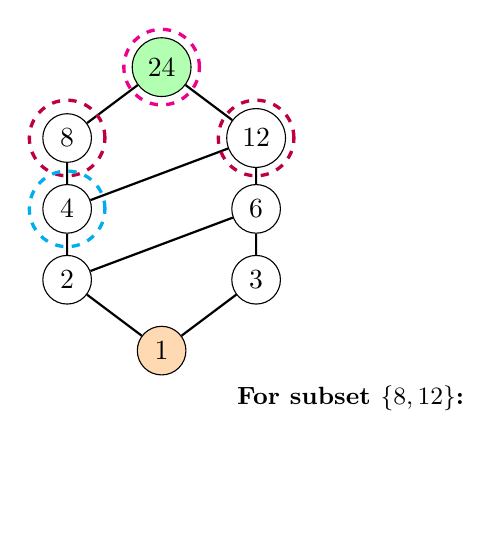
\begin{tikzpicture}[scale=0.6,
    every node/.style={circle, draw, fill=white, minimum size=6mm},
    minimal/.style={fill=red!30},
    maximal/.style={fill=blue!30},
    least/.style={fill=orange!30},
    greatest/.style={fill=green!30}]
    
    % Nodes
    \node[least] (1) at (0,0) {1};
    \node (2) at (-2,1.5) {2};
    \node (3) at (2,1.5) {3};
    \node (4) at (-2,3) {4};
    \node (6) at (2,3) {6};
    \node (8) at (-2,4.5) {8};
    \node (12) at (2,4.5) {12};
    \node[greatest] (24) at (0,6) {24};
    
    % Edges
    \draw[thick] (1) -- (2);
    \draw[thick] (1) -- (3);
    \draw[thick] (2) -- (4);
    \draw[thick] (2) -- (6);
    \draw[thick] (3) -- (6);
    \draw[thick] (4) -- (8);
    \draw[thick] (4) -- (12);
    \draw[thick] (6) -- (12);
    \draw[thick] (8) -- (24);
    \draw[thick] (12) -- (24);
    
    % Highlight bounds for {8,12}
    \draw[dashed, purple, very thick] (8) circle (8mm);
    \draw[dashed, purple, very thick] (12) circle (8mm);
    \draw[dashed, cyan, very thick] (4) circle (8mm);
    \draw[dashed, magenta, very thick] (24) circle (8mm);
    
    % Labels
    \node[draw=none, fill=none] at (4,-1) {\small\textbf{For subset $\{8,12\}$:}};
\end{tikzpicture}
\end{center}

\textbf{Definitions:}

\textbf{\textcolor{red}{Minimal element}}: Elements at top or bottom with no elements below (e.g., 1)

\textbf{\textcolor{blue}{Maximal element}}: Elements at top or bottom with no elements above (e.g., 24)

\textbf{\textcolor{orange}{Least element}}: Unique element below all others - alone at top (1 is least)

\textbf{\textcolor{green}{Greatest element}}: Unique element above all others - alone at bottom (24 is greatest)

\textbf{\textcolor{cyan}{Lower bound}}: For subset $\{8,12\}$, element where $\ell | 8$ and $\ell | 12$ (here: 1,2,4)

\textbf{\textcolor{purple}{Upper bound}}: For subset $\{2,3\}$, element where $2|u$ and $3|u$ (here: 6,12,24)

\textbf{\textcolor{cyan}{Greatest lower bound (GLB/meet)}}: Largest lower bound = $\gcd(8,12) = 4$

\textbf{\textcolor{magenta}{Least upper bound (LUB/join)}}: Smallest upper bound = $\text{lcm}(8,12) = 24$

\textbf{Note:} With divisibility relation, there would be no least element without 1!

\subsection*{Euler's $\phi$ Function Table}

{\tiny
\setlength{\tabcolsep}{2pt}
\begin{tabular}{|c|c||c|c||c|c||c|c||c|c||c|c|}
\hline
$n$ & $\phi$ & $n$ & $\phi$ & $n$ & $\phi$ & $n$ & $\phi$ & $n$ & $\phi$ & $n$ & $\phi$ \\
\hline
1 & 1 & 21 & 12 & 41 & 40 & 61 & 60 & 81 & 54 & 101 & 100 \\
2 & 1 & 22 & 10 & 42 & 12 & 62 & 30 & 82 & 40 & 102 & 32 \\
3 & 2 & 23 & 22 & 43 & 42 & 63 & 36 & 83 & 82 & 103 & 102 \\
4 & 2 & 24 & 8 & 44 & 20 & 64 & 32 & 84 & 24 & 104 & 48 \\
5 & 4 & 25 & 20 & 45 & 24 & 65 & 48 & 85 & 64 & 105 & 48 \\
6 & 2 & 26 & 12 & 46 & 22 & 66 & 20 & 86 & 42 & 106 & 52 \\
7 & 6 & 27 & 18 & 47 & 46 & 67 & 66 & 87 & 56 & 107 & 106 \\
8 & 4 & 28 & 12 & 48 & 16 & 68 & 32 & 88 & 40 & 108 & 36 \\
9 & 6 & 29 & 28 & 49 & 42 & 69 & 44 & 89 & 88 & 109 & 108 \\
10 & 4 & 30 & 8 & 50 & 20 & 70 & 24 & 90 & 24 & 110 & 40 \\
11 & 10 & 31 & 30 & 51 & 32 & 71 & 70 & 91 & 72 & 111 & 72 \\
12 & 4 & 32 & 16 & 52 & 24 & 72 & 24 & 92 & 44 & 112 & 48 \\
13 & 12 & 33 & 20 & 53 & 52 & 73 & 72 & 93 & 60 & 113 & 112 \\
14 & 6 & 34 & 16 & 54 & 18 & 74 & 36 & 94 & 46 & 114 & 36 \\
15 & 8 & 35 & 24 & 55 & 40 & 75 & 40 & 95 & 72 & 115 & 88 \\
16 & 8 & 36 & 12 & 56 & 24 & 76 & 36 & 96 & 32 & 116 & 56 \\
17 & 16 & 37 & 36 & 57 & 36 & 77 & 60 & 97 & 96 & 117 & 72 \\
18 & 6 & 38 & 18 & 58 & 28 & 78 & 24 & 98 & 42 & 118 & 58 \\
19 & 18 & 39 & 24 & 59 & 58 & 79 & 78 & 99 & 60 & 119 & 96 \\
20 & 8 & 40 & 16 & 60 & 16 & 80 & 32 & 100 & 40 & 120 & 32 \\
\hline
\end{tabular}
}

\textbf{Quick pattern:} $6 \cdot 11 \equiv_{13} 1$ (from mod table)

\end{multicols}
\end{document}
